Kapittelet vil gi en kort presentasjon av konsernet og datterselskapet AS ROCKWOOL. Videre vil det redegjøres for nåsituasjonen til Rockwool, og hvilke utfordringer virksomheten står overfor i dag.

\section{Om selskapet}
ROCKWOOL International er verdens største steinullprodusent med over 11.000 ansatte fordelt på salgskontorer og fabrikker i 39 land. Virksomheten baseres på utvinning av vulkansk stein for å produsere produkter, systemer og løsninger innenfor byggisolasjon. Selskapet hadde i 2018 salgsinntekter på 26,149 milliarder kroner og et årsresultat på 2,064 milliarder kroner \cite{annualReport}.

\subsection{AS ROCKWOOL}
AS ROCKWOOL er et heleid norsk datterselskap av ROCKWOOL international. Virksomhetens visjon er \textit{“AS ROCKWOOL skal være ledende leverandør av isolasjon, der positivt bidrag til et bedre miljø og brannsikring skal være førende”}. Datterselskapet består av 240 ansatte fordelt på to fabrikker og et salgskontor. Disse er lokalisert i henholdsvis Moss, Trondheim og Oslo. I 2018 hadde de salgsinntekter på 919 millioner kroner og leverte et årsresultat på litt over 86 millioner kroner \cite{osloRegnskap}.

\indent \newline
Produksjonsprosessen foregår ved at vulkansk stein og koks blir tilsatt i den varme enden av maskinen og deretter utsatt for enormt høye temperaturer i en smelteovn. Videre blir det tilsatt bindemiddel hvor den glødende massen blir omgjort til ullfibre før massen spinnes til steinull.

\begin{figure}[H]
\centering
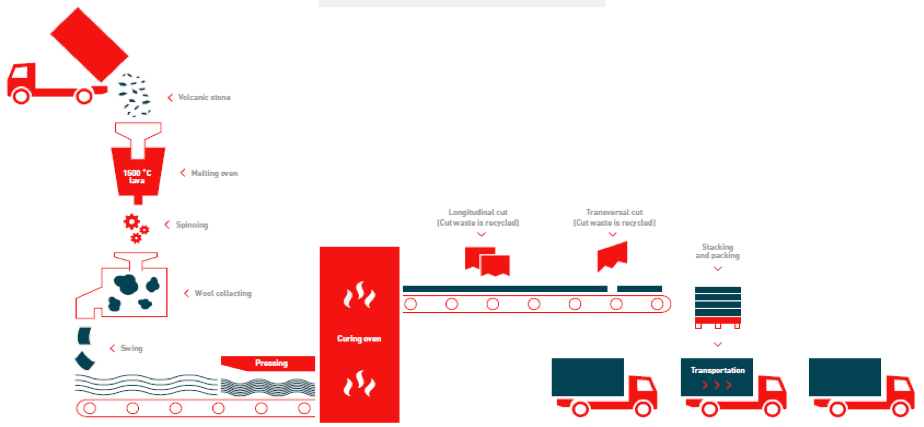
\includegraphics [scale=0.95]{bilder/produksjonsprosess.png}
\caption{Produksjonsprosess}
\label{fig:produksjonsprosess}
\end{figure}

\section{Historie}
I 1937 ble den første Rockwool-fabrikken etablert i Danmark. Få år senere utvidet konsernet med fabrikker i Larvik, Trondheim og Moss. Siden oppstarten i Norge har Rockwool basert virksomheten på utvinning av vulkansk stein, hvor produksjonsprosessen har forandret seg lite. Imidlertid investerte de nærmere en halv milliard kroner i nytt produksjonsutstyr på fabrikken i Moss i 2002, med et formål om å automatisere produksjonen. Dette har ført til mer enn en fordobling av produksjonskapasiteten. I løpet av de siste årene har de innført en lean-metode som de kaller for Ropex, med et ønske om å effektivisere virksomheten gjennom hele verdikjeden \cite{dagsavisen}.

\indent \newline
I 2016 vedtok Rockwool-konsernet å forplikte seg til FNs bærekraftsmål, hvorav 6 av 10 er implementert som interne konsernmål. Målene representerer forbedringer innenfor sikkerhet og helse, vannforbruk, energieffektivitet, avfallsresirkulering, og reduksjon i avfall og CO2-utslipp i produksjonsprosessen. Ett av målene er å redusere CO2-utslippet med 10\% innen 2022 og 20\% innen 2030.

\begin{figure}[H]
\centering
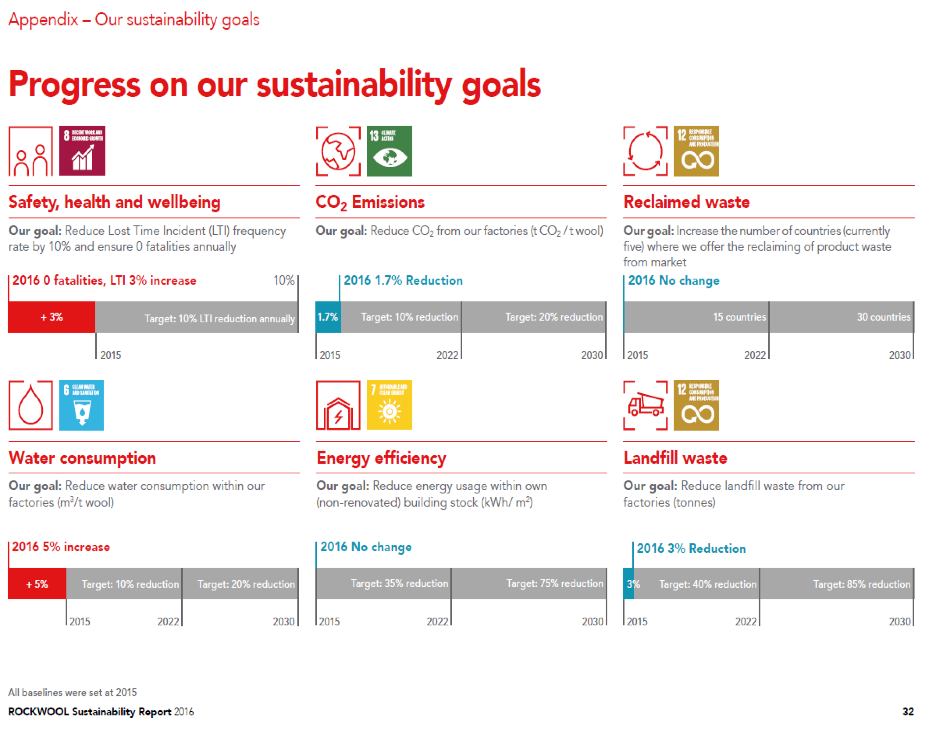
\includegraphics [scale=0.9]{bilder/baerkraftsmal.png}
\caption{Bærekraftsmål}
\label{fig:baerkraftsmal}
\end{figure}

\section{Markedet i Norge}  
Byggisolasjonsbransjen består av noen få store aktører som i likhet med Rockwool er datterselskaper av verdensomspennende konsern. Markedet karakteriseres av store mobilitetsbarrierer gjennom krav til kapitalintensive investeringer i spesialisert produksjonsutstyr. Rockwool har i flere år levert gode resultater, og er i dag markedets nest største aktør med en markedsandel på rundt 26\%. De mest nærliggende konkurrentene er Glava, Knauf, Sundolitt og Paroc, hvor Glava er markedets største med en markedsandel på 40\%. Kundene består i hovedsak av byggevarekjeder og entreprenører og sitter med høy forhandlingsmakt i form av at produsentene tilbyr lite differensierte produkter. Imidlertid leverer Rockwool og Paroc de mest differensierte produktene i form av produktegenskapene. De to virksomhetene er de eneste produsentene som leverer produkter som isolerer, er vannavstøtende, har lyddempende egenskaper og som er en god kilde til brannsikring. 

\indent \newline
Markedsveksten ligger på rundt 2\% og forventes å ligge på samme nivå i årene fremover. Dette viser til et modent marked. Den siste tiden har imidlertid Rockwool opplevd en lavere prosentvis vekst, grunnet en utvikling i markedet hvor miljøet blir vektlagt mer enn tidligere. Det blir vanligere for entreprenørene å BREEAM-sertifisere prosjektene sine. BREEAM er et miljøsertifiseringsverktøy for bygninger som legger vekt på miljøpåvirkning innenfor emner som energibruk, transport, materialer, avfall og forurensning\cite{breeam}. Dette påvirker spesielt produksjonsprosessen til isolasjonsprodusentene ved å stille krav til lavere utslipp. Rockwool sin nåværende smelteteknologi gir et høyere utslipp enn flere av konkurrentene, og er dermed en svakhet for virksomheten i forhold til å bli en foretrukken leverandør. 

\indent \newline
Det finnes også et annet økonomisk insentiv for produsentene til å redusere CO2-utslippet. Gjennom EØS-avtalen er Norge en del av Det europeiske kvotesystemet. Produsentene blir tildelt et visst antall kvoter og må kjøpe mer hvis utslippet overskrider det de får tildelt. Reduksjon i CO2-utslipp vil derfor resultere i lavere kostnader knyttet til drift.